% Chapter 4

\chapter{Experimental Results} % Main chapter title

\label{Chapter4} % For referencing the chapter elsewhere, use \ref{Chapter4} 
In this chapter we begin with a qualitative analysis of the posterior topic distributions generated by the DTM and inspect the historical significance and context of patents with particularly high inferred influence from the DIM. More quantitatively, we then present results from evaluating the coherence of each model's topics. Following the results of coherence testing we show the results of document classification via the document topic vectors produced by each of the three models. We conclude this chapter by presenting the performance of K-means clustering on each of the document vector spaces as measured by the metrics described in section \ref{DocumentClustering}.


%----------------------------------------------------------------------------------------
\section{Qualitative analysis of topics}
% Illustrate the progression of a topic through time
% Identify influential patents to a topic and assess their historical importance to the field.
%

%stream and damless patents, check out word progression
The experimental results show that both the DTM and DIM successfully identify latent topic structures consistent with known industry history. As an example we inspect the topic generated by the DTM most closely associated with the "Stream and Damless" hydro power CPC patent subclass (those with the label \keyword{YO2E 10$/$28}). Figure \ref{fig:areaplot} illustrates the mean topic vector for documents of this CPC subclass across epochs, primarily dominated by topic 4. If we inspect the top words from the inferred posterior distribution of this topic, shown in figure \ref{fig:wwttTopic4}, we see that while central words such as "water" and "power" maintain a high likelihood, words such as "float" experience an increase in likelihood as time progresses. 

% area chart of cumulative topic percentages in class over time. (i.e. add up all the vectors, normalize ot total amount, find percent, repeat for each epoch.)
\begin{figure}[!htb]
\centering
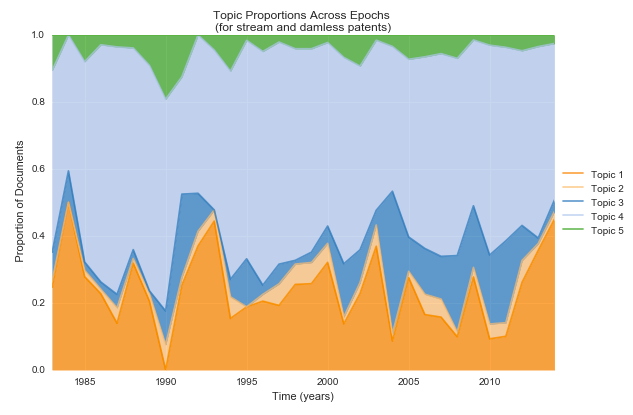
\includegraphics[width=130mm,scale=0.45]{Figures/areaplot2}
\decoRule
\caption[areaplot]{Proportion of topics at each epoch for patents relating to stream and damless hydro electric technology}
\label{fig:areaplot}
\end{figure}

% This parallels an increase in offshore floating barge popularity 
To understand why this might be the case we reviewed the known history of stream and damless hydro technology, and found that the increase of the word "float" is of particular interest as it parallels closely the development of the wave and tidal energy industry both in the UK and globally. Vertical cross flow turbines such as the Gorlov turbine, patented in 2001, contributed to a rise in the popularity of floating barges for tidal power, a technology that represents the current norm of tidal current development \parencite{KhanOES}. Closely following this the European Marine Energy Centre (\keyword{EMEC}) was founded in 2003 and since then has supported the deployment of more wave and tidal energy devices than at any other single site in the world. This substantiates the linguistic trends we observe in Topic 4 and offers an explanation as to the rise in the estimated posterior mean number of occurrences of words such as "power" and "float" after 2003.

% also reflected in the importances of certain patents
Additionally, inspecting the patents in the "Stream and Damless" subclass that were estimated by the DIM as having a particularly high influence to Topic 4 reveals a similar narrative. During the same period of growth for barge based systems as discussed above, beginning around the year 2000, we see the DIM infer linguistic importance to related patents. For instance, a buoyancy pump in 2000, an energy generating method and device for utilizing buoyancy in 2006 and a cross flow hydraulic turbine in 2007 all received the largest influence scores of their epoch, a metric shown to correlate with forward citation rates \parencite{icml2010_GerrishB10}. In this way we are able, \emph{without} knowledge of citation rates, i.e. solely through analyzing language use, to identify individual patents likely to have had an influence on the terminology of the field in which they were published. 

%posterior distribution of the corpus' patent influences


% word distributions of topic 4 over time plot (the topic most closely associated with the cpc label 28)
\begin{figure}[!htb]
\centering
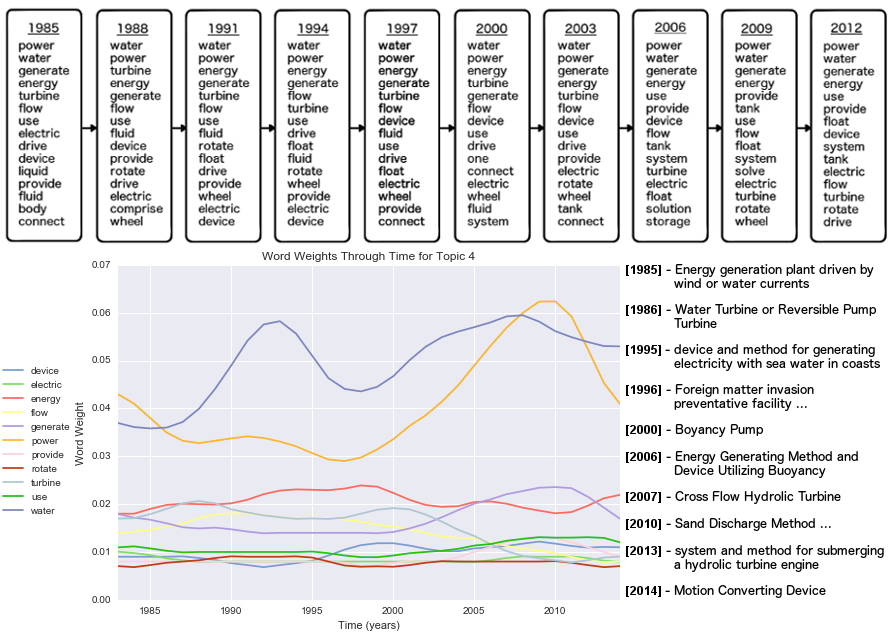
\includegraphics[width=130mm,scale=0.45]{Figures/Topic4}
\decoRule
\caption[wwttTopic4]{(top) The top fifteen words from the inferred posterior distribution of Topic 4 at three year lags. (bottom) The posterior estimate of the frequency as a function of year of words from Topic 4. (right) Patents of linguistic influence to topic across epochs as estimated by the DIM.}
\label{fig:wwttTopic4}
\end{figure}

%----------------------------------------------------------------------------------------
%\section{DIM Results and Insights}
%\subsection{Influence Metric}
%\subsubsection{validating influential patents}
%\subsubsection{correlation with forward citations}
%\subsubsection{correlation with page-rank}

%----------------------------------------------------------------------------------------
\section{Coherence Testing}
\label{coherencetesting}

The aggregated topic coherence results of the tuned models are shown in Table \ref{tab:coherences} for the DTM, DIM and LDA models respectively.

When testing the coherence of each model's topics, the DTM proved superior in all coherence measures except Umass, the measure that correlates the least with human judgement by a considerable amount. Not only did the DTM regularly obtain the highest coherence scores, it did so by a large margin obtaining nearly double the c$\_$uci score obtained by static LDA. We attribute this performance to the unique structure of the DTM. Rather than enforcing broad sweeping "one size fits all" topics across the whole corpus as with traditional LDA, with the DTM each epoch receives in effect its own LDA model. Each of these individual LDA models inherits a set of variational parameters $\alpha$ and $\beta$, from the previous time step that have been perturbed by Gaussian noise and control its document topic-proportions and topic word-distributions respectively. The result is a richer posterior compared to static LDA that allows for a 'tighter fit' to the true posterior. This naturally takes longer to train but is demonstrably worth the performance increase.


Though the DIM received the highest U$\_$mass score, it is interesting to note that for the most part the DIM obtained coherence scores similar to, but consistently smaller than, that of its counterpart the DTM. This is again due to the structure of the model. The DIM borrows a similar Markov chain structure of word distributions in order to capture drifts in probabilities over the course of the document collection, but with one critical difference. While the topic word-distribution natural parameters $\beta$ are passed along at each time step the DIM does not chain its document topic-proportion natural parameters $\alpha$. Thus each epoch's LDA operates under the same $\alpha$ parameters which weakens its ability to superresolve temporal topic trends. This explains the increased performance of the DIM over traditional LDA, and reduced performance compared to the DTM. 

\begin{table}[!htb]
\caption[Coherences]{The coherence values attained by each model}
\label{tab:coherences}
\centering
\begin{tabular}{l l l l l}
\toprule
\tabhead{Model} & \tabhead{c$\_$v} & \tabhead{c$\_$uci} & \tabhead{c$\_$npmi} & \tabhead{u$\_$mass} \\
\midrule
LDA & .5021 & .1904 & .0750 & -1.6283 \\
DIM & .5581 & .2865 & .1011 & \keyword{-1.3478} \\
DTM & \keyword{.5980} & \keyword{.4373} & \keyword{.1213} & -1.6688 \\
\bottomrule\\
\end{tabular}
\end{table}

Results are analogous when looking at coherences across epochs, illustrated in figure \ref{fig:EpochCoherences}, as opposed to the aggregated coherence scores. As the static LDA produced only a single set of topics for the entire corpus its coherence scores remain constant. The DTM however provided unique topics across epochs and thus obtained a sequence of coherence scores. This sequence of scores contained minor fluctuations but again persistently remained above those of the static LDA model for all measures except Umass.
 
 %Again, Umass gives less conclusive results than the other metrics. 

\begin{figure}[!htb]
\centering
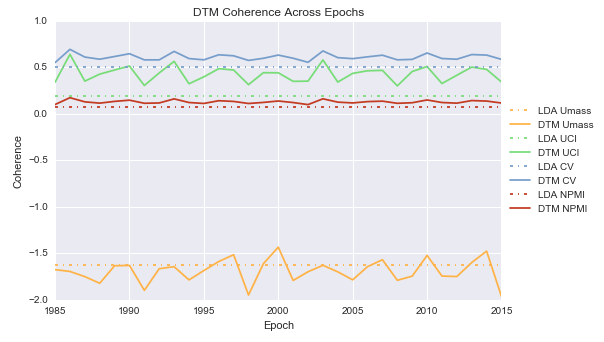
\includegraphics[width=130mm,scale=0.45]{Figures/DTMCoherences}
\decoRule
\caption[EpochCoherences]{Coherence scores for the DTM and LDA across epochs}
\label{fig:EpochCoherences}
\end{figure}


%----------------------------------------------------------------------------------------
\section{Classification Results}
\label{classres}
At classification the DTM again proved superior, with a final precision, recall and F1 score of .64, .64, and .64 respectively. However the DIM performed marginally worse than the static LDA model, a contrast to the DIM's improved topic coherences compared to static LDA. The DIM generated a final precision, recall, and F1 score of .58, .56, and .56 while the static LDA model yielded precision, recall and F1 scores of .58, .58, and .58.

Table \ref{tab:classifiers} contains the cross validated F1 scores of each classifier trained on the document topic vectors provided by static LDA, the DTM and DIM. We used radial basis function support vector machines to generate the final classification results as this classifier yielded the highest cross validated F1 score across all three models.

The precision, recall, and F1 score for LDA, DIM and the DTM, broken down by patent class labels, can be found in tables \ref{tab:ldaclass}, \ref{tab:dimclass}, and \ref{tab:dtmclass} respectively. These results are illustrated in their corresponding normalized confusion matrices found in figures \ref{fig:LDAmatrix}, \ref{fig:DIMmatrix}, and \ref{fig:DTMmatrix}. Patents relating to "turbines and wheels" tended to be the most difficult to classify while "conventional" patents were generally the best classified. The precision and recall was reasonably balanced for the classifiers of all three models, with the DIM based classifier favoring precision slightly. 

%samples aren't balanced so we considered f1 score rather than just accuracy.

\begin{table}[!htb]
\caption[crossvalclass]{Cross validated accuracy score for each classifier}
\label{tab:classifiers}
\centering
\begin{tabular}{l  l  l  l}
\toprule
\tabhead{Model} & \tabhead{DTM CV score} & \tabhead{DIM CV score}  & \tabhead{LDA CV Score} \\
\midrule
ASGD & 0.621013 & 0.521755 & 0.556590 \\
Adaboost & 0.567315 & 0.504048 & 0.514788 \\
Decision Tree & 0.491707 & 0.546153 & 0.490798 \\
Gaussian NB & 0.582415 & 0.540346 & 0.530325 \\
KNN & 0.553341 & 0.472817 & 0.494431 \\
LDA & 0.618973 & 0.534562 & 0.551576 \\
LR & 0.620385 & 0.521948 & 0.555715 \\
Lin. SVC & 0.564651 & 0.447450 & 0.510240 \\
Passive-Aggressive I & 0.601775 & 0.506445 & 0.450347 \\
Passive-Aggressive II & 0.385359 & 0.378960 & 0.397031 \\
Perceptron & 0.458625 & 0.379983 & 0.434744 \\
QDA & 0.585174 & 0.453922 & 0.529446 \\
RBF SVM & \keyword{0.637477} & \keyword{0.564730} & \keyword{0.578102} \\
Random Forest & 0.524156 & 0.547191 & 0.472841 \\
SGD & 0.602344 & 0.514596 & 0.550329 \\
\bottomrule\\
\end{tabular}
\end{table}


%-----------lda classification table----------------------

\begin{table}[!htb]
\caption[ldaclass]{Classification results of LDA based classifier}
\label{tab:ldaclass}
\centering
\begin{tabular}{l l l l}
\toprule
\tabhead{Class Label} & \tabhead{Precision} & \tabhead{Recall} & \tabhead{F1} \\
\midrule
 Hydro energy & 0.49 & 0.52 & 0.50 \\
 Conventional & 0.62 & 0.65 & 0.64 \\
 Turbines and Wheels & 0.45 & 0.44 & 0.44  \\
 Other Parts & 0.61 & 0.57 & 0.59  \\
 Stream and Damless & 0.63 & 0.62 & 0.62  \\
\hline 
 Avg$/$Total & 0.58 & 0.58 & 0.58  \\
\bottomrule\\
\end{tabular}
\end{table}

\newpage

%-----------dim classification table----------------------
\begin{table}[!htb]
\caption[ldaclass]{Classification results of DIM based classifier}
\label{tab:dimclass}
\centering
\begin{tabular}{l l l l}
\toprule
\tabhead{Class Label} & \tabhead{Precision} & \tabhead{Recall} & \tabhead{F1} \\
\midrule
Hydro energy  & 0.38 & 0.44 & 0.41 \\
       Conventional  & 0.68 & 0.60 & 0.63 \\
Turbines and Wheels  & 0.42 & 0.43 & 0.43 \\
        Other Parts  & 0.56 & 0.66 & 0.61 \\
 Stream and Damless  & 0.68 & 0.53 & 0.59 \\
\hline
 Avg$/$Total & 0.58 & 0.56 & 0.56 \\
\bottomrule\\
\end{tabular}
\end{table}

%-----------dtm classification table----------------------
\begin{table}[!htb]
\caption[dtmclass]{Classification results of DTM based classifier}
\label{tab:dtmclass}
\centering
\begin{tabular}{l l l l}
\toprule
\tabhead{Class Label} & \tabhead{Precision} & \tabhead{Recall} & \tabhead{F1} \\
\midrule
Hydro energy & 0.70 & 0.65 & 0.67 \\
       Conventional & 0.69 & 0.69 & 0.69 \\
Turbines and Wheels & 0.49 & 0.50 & 0.49 \\
        Other Parts & 0.63 & 0.62 & 0.63 \\
 Stream and Damless & 0.66 & 0.69 & 0.67 \\
\hline
 Avg$/$Total & 0.64 & 0.64 & 0.64 \\
\bottomrule\\
\end{tabular}
\end{table}

%-----------classification figures----------------------
\begin{figure}[!htb]
\centering
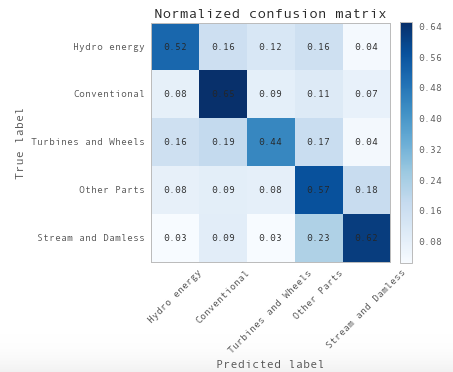
\includegraphics[scale=0.65]{Figures/ldaclass}
\decoRule
\caption[ldaclass]{Confusion matrix of LDA classification results}
\label{fig:LDAmatrix}
\end{figure}

\newpage 

\begin{figure}[!htb]
\centering
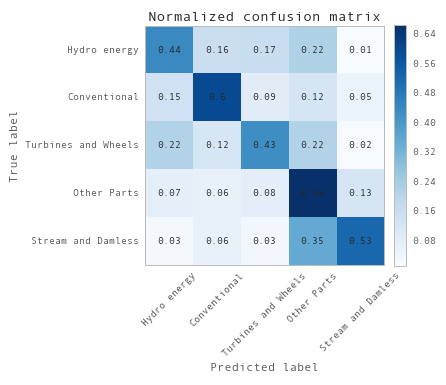
\includegraphics[scale=0.65]{Figures/dimclass}
\decoRule
\caption[dimclass]{Confusion matrix of DIM classification results}
\label{fig:DIMmatrix}
\end{figure}

\begin{figure}[!htb]
\centering
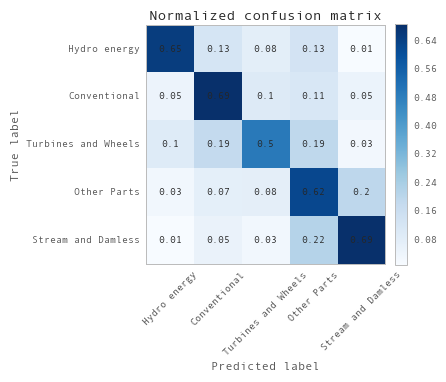
\includegraphics[scale=0.65]{Figures/dtmclass}
\decoRule
\caption[dtmclass]{Confusion matrix of DTM classification results}
\label{fig:DTMmatrix}
\end{figure}


\section{Clustering Results}
\label{clusres}
Here, we found that the vector spaces created by the DIM, and particularly the DTM, also excelled at effectively clustering documents. Scores for the various clustering metrics we calculated can be found in table \ref{tab:clusters}. The DTM received the highest silhouette score at .55, more than double the score of .22 received by LDA, meaning it provided the densest and most distinct clustering of the documents irrespective of their class labels.

When we take into account the true class labels of each patent, using the normalized mutual information (NMI), we see that the DTM again produces the highest score. This suggests a higher agreement between the DTM's K-means predicted labels and the true labels compared to those of the other models. However, the DIM achieved the highest adjusted rand index (ARI) of the three models indicating a high similarity between its K-means predicted labels and the true labels as well. Irrespective of this, the traditional static LDA received both the lowest NMI and ARI scores.

Finally, we observed that the dynamic models both produced higher homogeneity and completeness scores than the static LDA model, with the DTM again leading slightly over the DIM. The DTM achieved a homogeneity of .21 indicating that its corresponding kmeans cluster assignments each contained more members of a single class than had the other models' cluster assignments. Additionally the completeness of the DTM, measuring how well all members of a given class are assigned to the same cluster, was the highest at .207 with the DIM \emph{just} behind at .205 and LDA at .175.

To visualize the vector spaces generated by each model we made use of a handful of embedding algorithms, namely t-Distributed Stochastic Neighbor Embedding (\keyword{t-SNE}) , Principle Component Analysis  (\keyword{PCA}), and Linear Discriminant Analysis (\keyword{LDA}), to project the spaces down to 2 dimensions. The results of this visualization can be seen in figure \ref{fig:clusterembeds}.
It is interesting to observe how strikingly different the vector spaces produced by the DTM, DIM and LDA model are when plotted side by side. However some themes run constant throughout such as the proximity of "turbines and wheels" and "other parts" patents, represented by the two shades of green. This is substantiated by the classification confusion matrices illustrated in section \ref{classres} where we see that classifiers tended to have difficulty in assigning labels for "turbines and wheels" and "other parts" patents, more commonly mistaking them for each other than for other classes.

\begin{table}[!htb]
\caption[Coherences]{Clustering results}
\label{tab:clusters}
\centering
\begin{tabular}{l l l l l}
\toprule
\tabhead{metric} & \tabhead{DTM} & \tabhead{DIM} & \tabhead{LDA} \\
\midrule
Silhouette   & 0.559518 & 0.370500 & 0.227973 \\
NMI	 		 & 0.210324 & 0.208029 	& 0.177195 \\
ARI		& 0.140005		& 0.158060		& 0.108182  \\
Homogeneity  & 0.213513 & 0.210767 & 0.178718 \\
Completeness & 0.207182 & 0.205327 & 0.175685 \\

\bottomrule\\
\end{tabular}
\end{table}


% they cite the normalized mutual information equation! use those!
%The clustering result is evaluated by comparing the Normalized mutual information (Xu et al. 2003; Cai et al. 2008) [NEED TO ACTUALLY CITE]


%Xu, W., Liu, X., & Gong, Y. (2003). Document clustering based on non-negative matrix factorization. In
%SIGIR ’03: Proceedings of the 26th annual international ACM SIGIR conference on research and
%development in informaion retrieval (pp. 267–273). New York, NY, USA: ACM.
%Cai, D., Mei, Q., Han, J., & Zhai, C. (2008). Modeling hidden topics on document manifold. In
%J. G. Shanahan, S. Amer-Yahia, I. Manolescu, Y. Zhang, D. A. Evans, A. Kolcz, K.-S. Choi, &
%A. Chowdhury (Eds.), CIKM (pp. 911–920). ACM.


\begin{figure}[!htb]
\centering
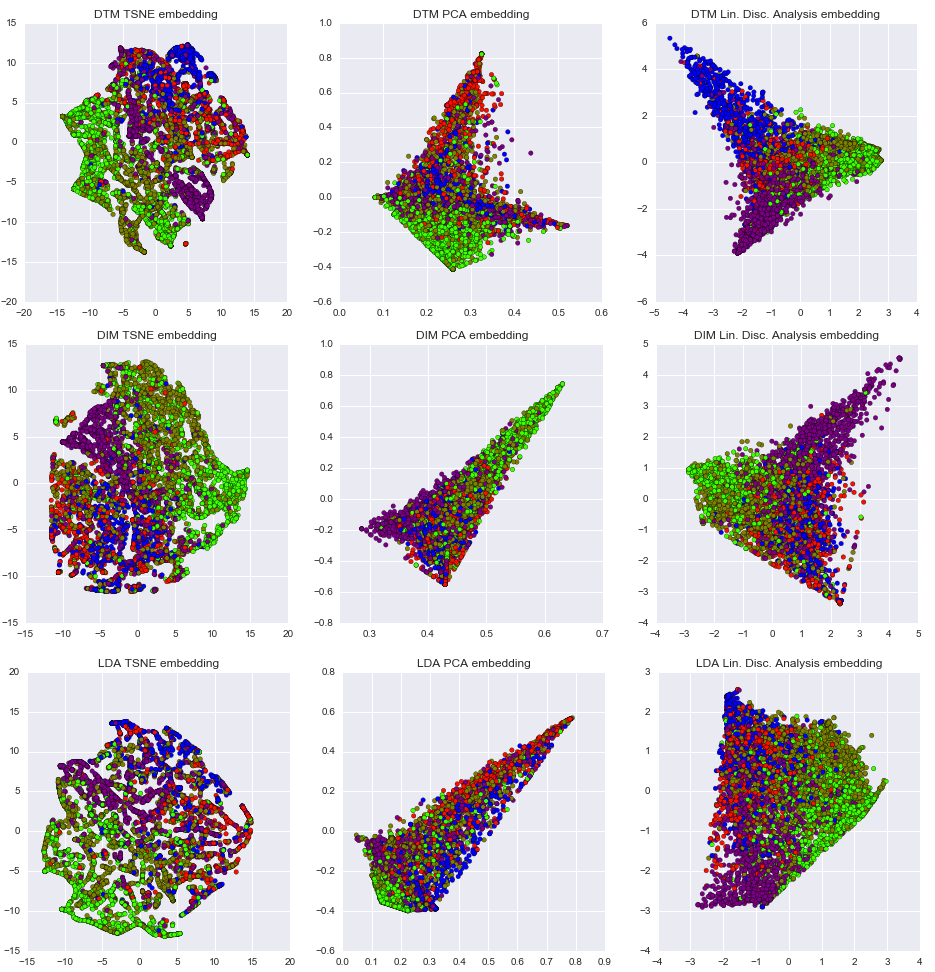
\includegraphics[width=130mm,scale=0.65]{Figures/Clusters}
\decoRule
\caption[clusterembeds]{TSNE, PCA and Linear Discriminant Analysis embeddings for the vector spaces generated by DTM, DIM, and LDA model}
\label{fig:clusterembeds}
\end{figure}